\section{Prior Work on Duality: Neural Path Framework}\label{sec:dual}
In this section, we will present a brief overview of dual view for fully connected DNN (FC-DNN) with ReLU as presented in [\citenum{npk}]. 

\subsection{Input Output Relationship in Fully Connected DNN: Primal View }
We consider fully-connected DNNs with `$w$' hidden units per layer and `$d-1$' hidden layers. $\Theta\in\R^{\dnet}$ are the network weights, where $\dnet=\din w+(d-2)w^2+w$. The information flow is shown in \Cref{tb:basic}, where
$\Theta(i,j,l)$ is the weight connecting the $j^{th}$ hidden unit of layer $l-1$ to the $i^{th}$ hidden unit of layer $l$. Further, $\Theta(\cdot,\cdot,1)\in\R^{w\times \din}, \Theta(\cdot,\cdot,l)\in\R^{w\times w},\forall l\in\{2,\ldots,d-1\}, \Theta(\cdot,\cdot,d)\in\R^{1\times w}$.
\begin{table}[h]
\centering
\begin{tabular}{|l l lll|}\hline
Input Layer&: &$z_{x,\Theta}(0)$ &$=$ &$x$ \\
Pre-Activation Input&: & $q_{x,\Theta}(i,l)$& $=$ & $\sum_{j} \Theta(i,j,l)\cdot z_{x,\Theta}(j,l-1)$\\
Gating Values&: &$G_{x,\Theta}(i,l)$& $=$ & $\mathbbm{1}_{\{q_{x,\Theta}(i,l)>0\}}$\\
Hidden Layer Output&: &$z_{x,\Theta}(i,l)$ & $=$ & $q_{x,\Theta}(i,l)\cdot G_{x,\Theta}(i,l)$ \\
Final Output&: & $\hat{y}_{\Theta}(x)$ & $=$ & $\sum_{j\in[w]} \Theta(1,j,d-1)\cdot z_{x,\Theta}(j,d-1)$\\\hline
\end{tabular}
\caption{Here, $l\in[d-1],i\in[w]$, $j\in[\din]$ for $l=1$ and $j\in[w]$ for $l=2,\ldots,d-1$.} 
\label{tb:basic}
\end{table}


\subsection{Encoding Gates and Weights: Neural Path Feature (NPF) and Neural Path Value (NPV)}
\begin{definition}
A path starts from an input node, passes through a weight and a hidden node in each layer and ends at the output node. We define the following quantities for a path $p$:
\begin{tabular}{lcl}
 Activity&:& $A_{\Theta}(x,p)$ is the product of the `$d-1$' gates in the path. \\
Value&:& $v_{\Theta}(p)$ is the product of the `$d$' weights in the path.\\
Feature&:&   $\phi_{x,\Theta}(p)$ is the product of the signal at the input node of the path and $A_{\Theta}(x,p)$.\\
\end{tabular}
\end{definition}
In a FC-DNN with `$d$' layers and  $w$  hidden units in each layer, there are $\Pfc=\din w^{(d-1)}$ paths. A path is active only if all the gates in the path are active.
\begin{figure}[h]
\resizebox{\columnwidth}{!}{
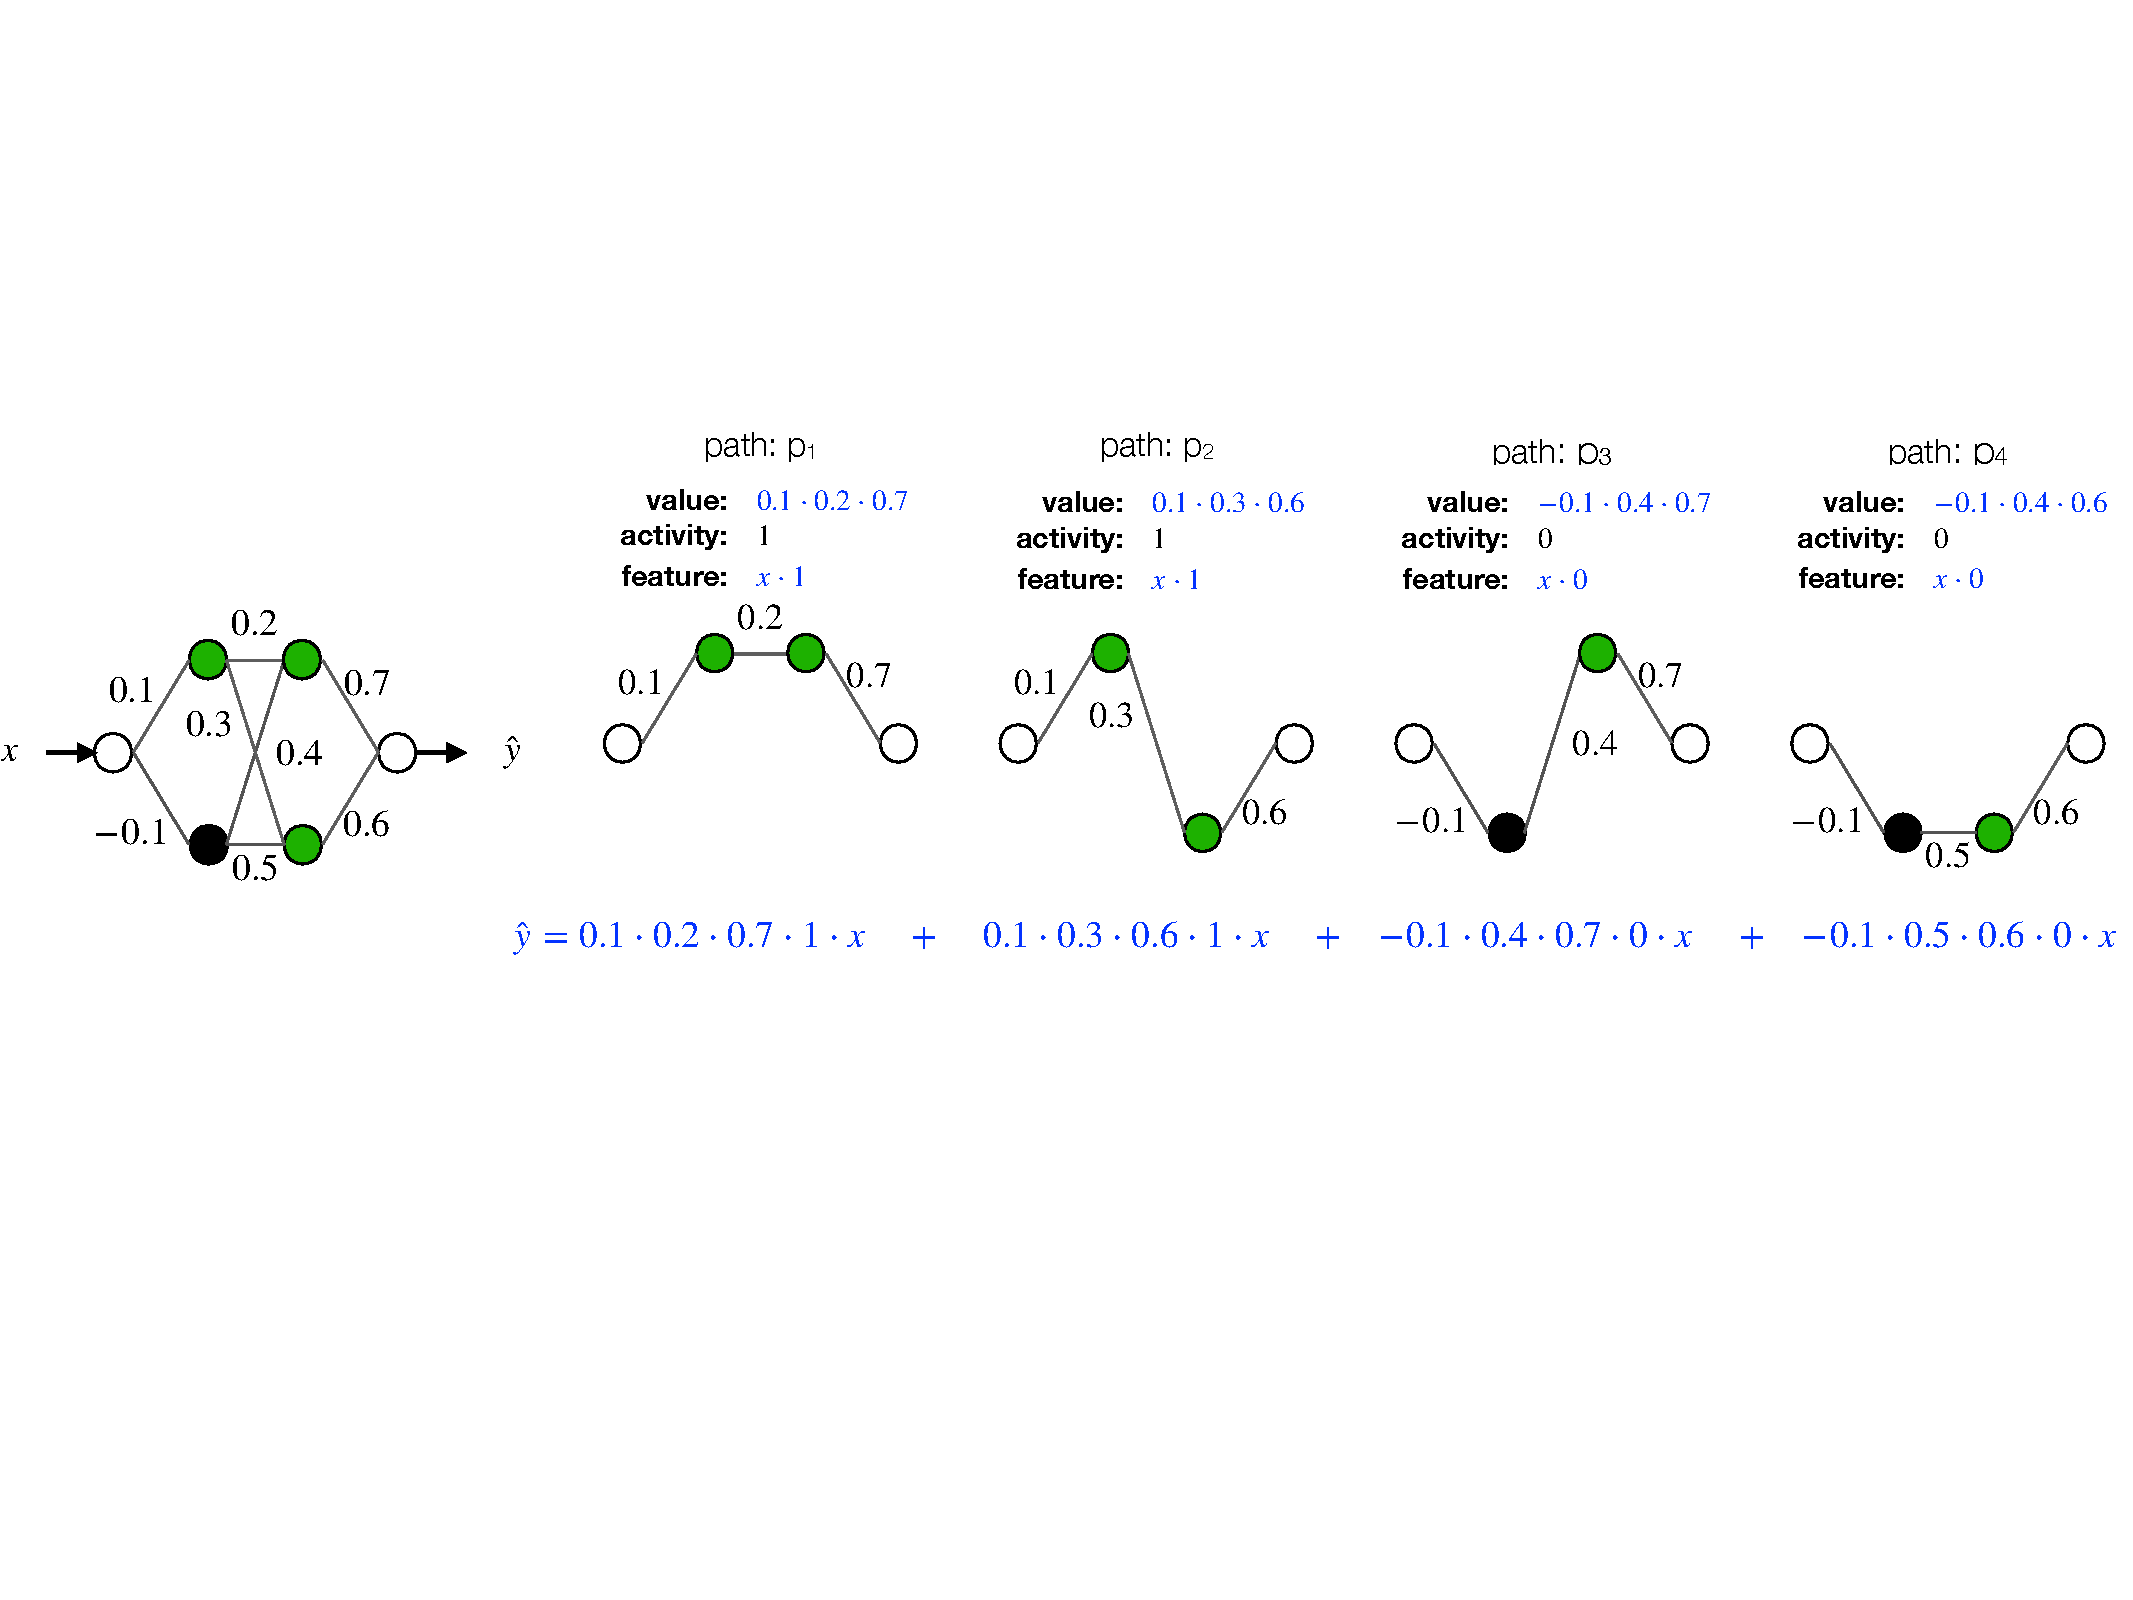
\includegraphics[scale=0.5]{figs/paths.pdf}
}
\caption{Shows a toy network with $2$ layers, $2$ gates per layer and $4$ paths. Paths $p_1$ and $p_2$ are `on' and paths $p_3$ and $p_4$ are `off'. The value, activity and feature of the individual paths are shown. The output $\hat{y}$ is the summation of the contributions of the individual paths.}
\end{figure}
\begin{proposition}
 Assuming that the paths can be enumerate as $1,\ldots, \Pfc$, one can collect the features and values of all the paths in the so called \emph{neural path feature} (NPF) given by $\phi_{x,\Theta}=\left(\phi_{x,\Theta}(p)\right),\in[\Pfc]$ and the \emph{neural path value} (NPV) given by $v_{\Theta}=\left(v_{\Theta}(p)\right),\in[\Pfc]$. The output of the DNN is then the inner product of the NPF and NPV, i.e., 
\begin{align}
\hat{y}_{\Theta}(x)=\ip{\phi_{x,\Theta},v_{\Theta}}=\sum_{p\in[P]}  \phi_{x,\Theta}(p) v_{\Theta}(p)
\end{align}
\end{proposition}


\subsection{Deep Gated Network : Decoupling Gates (NPV) and Weights (NPF) }\label{sec:dgn}
\begin{comment}
\begin{wrapfigure}{r}{0.3\textwidth}
\centering
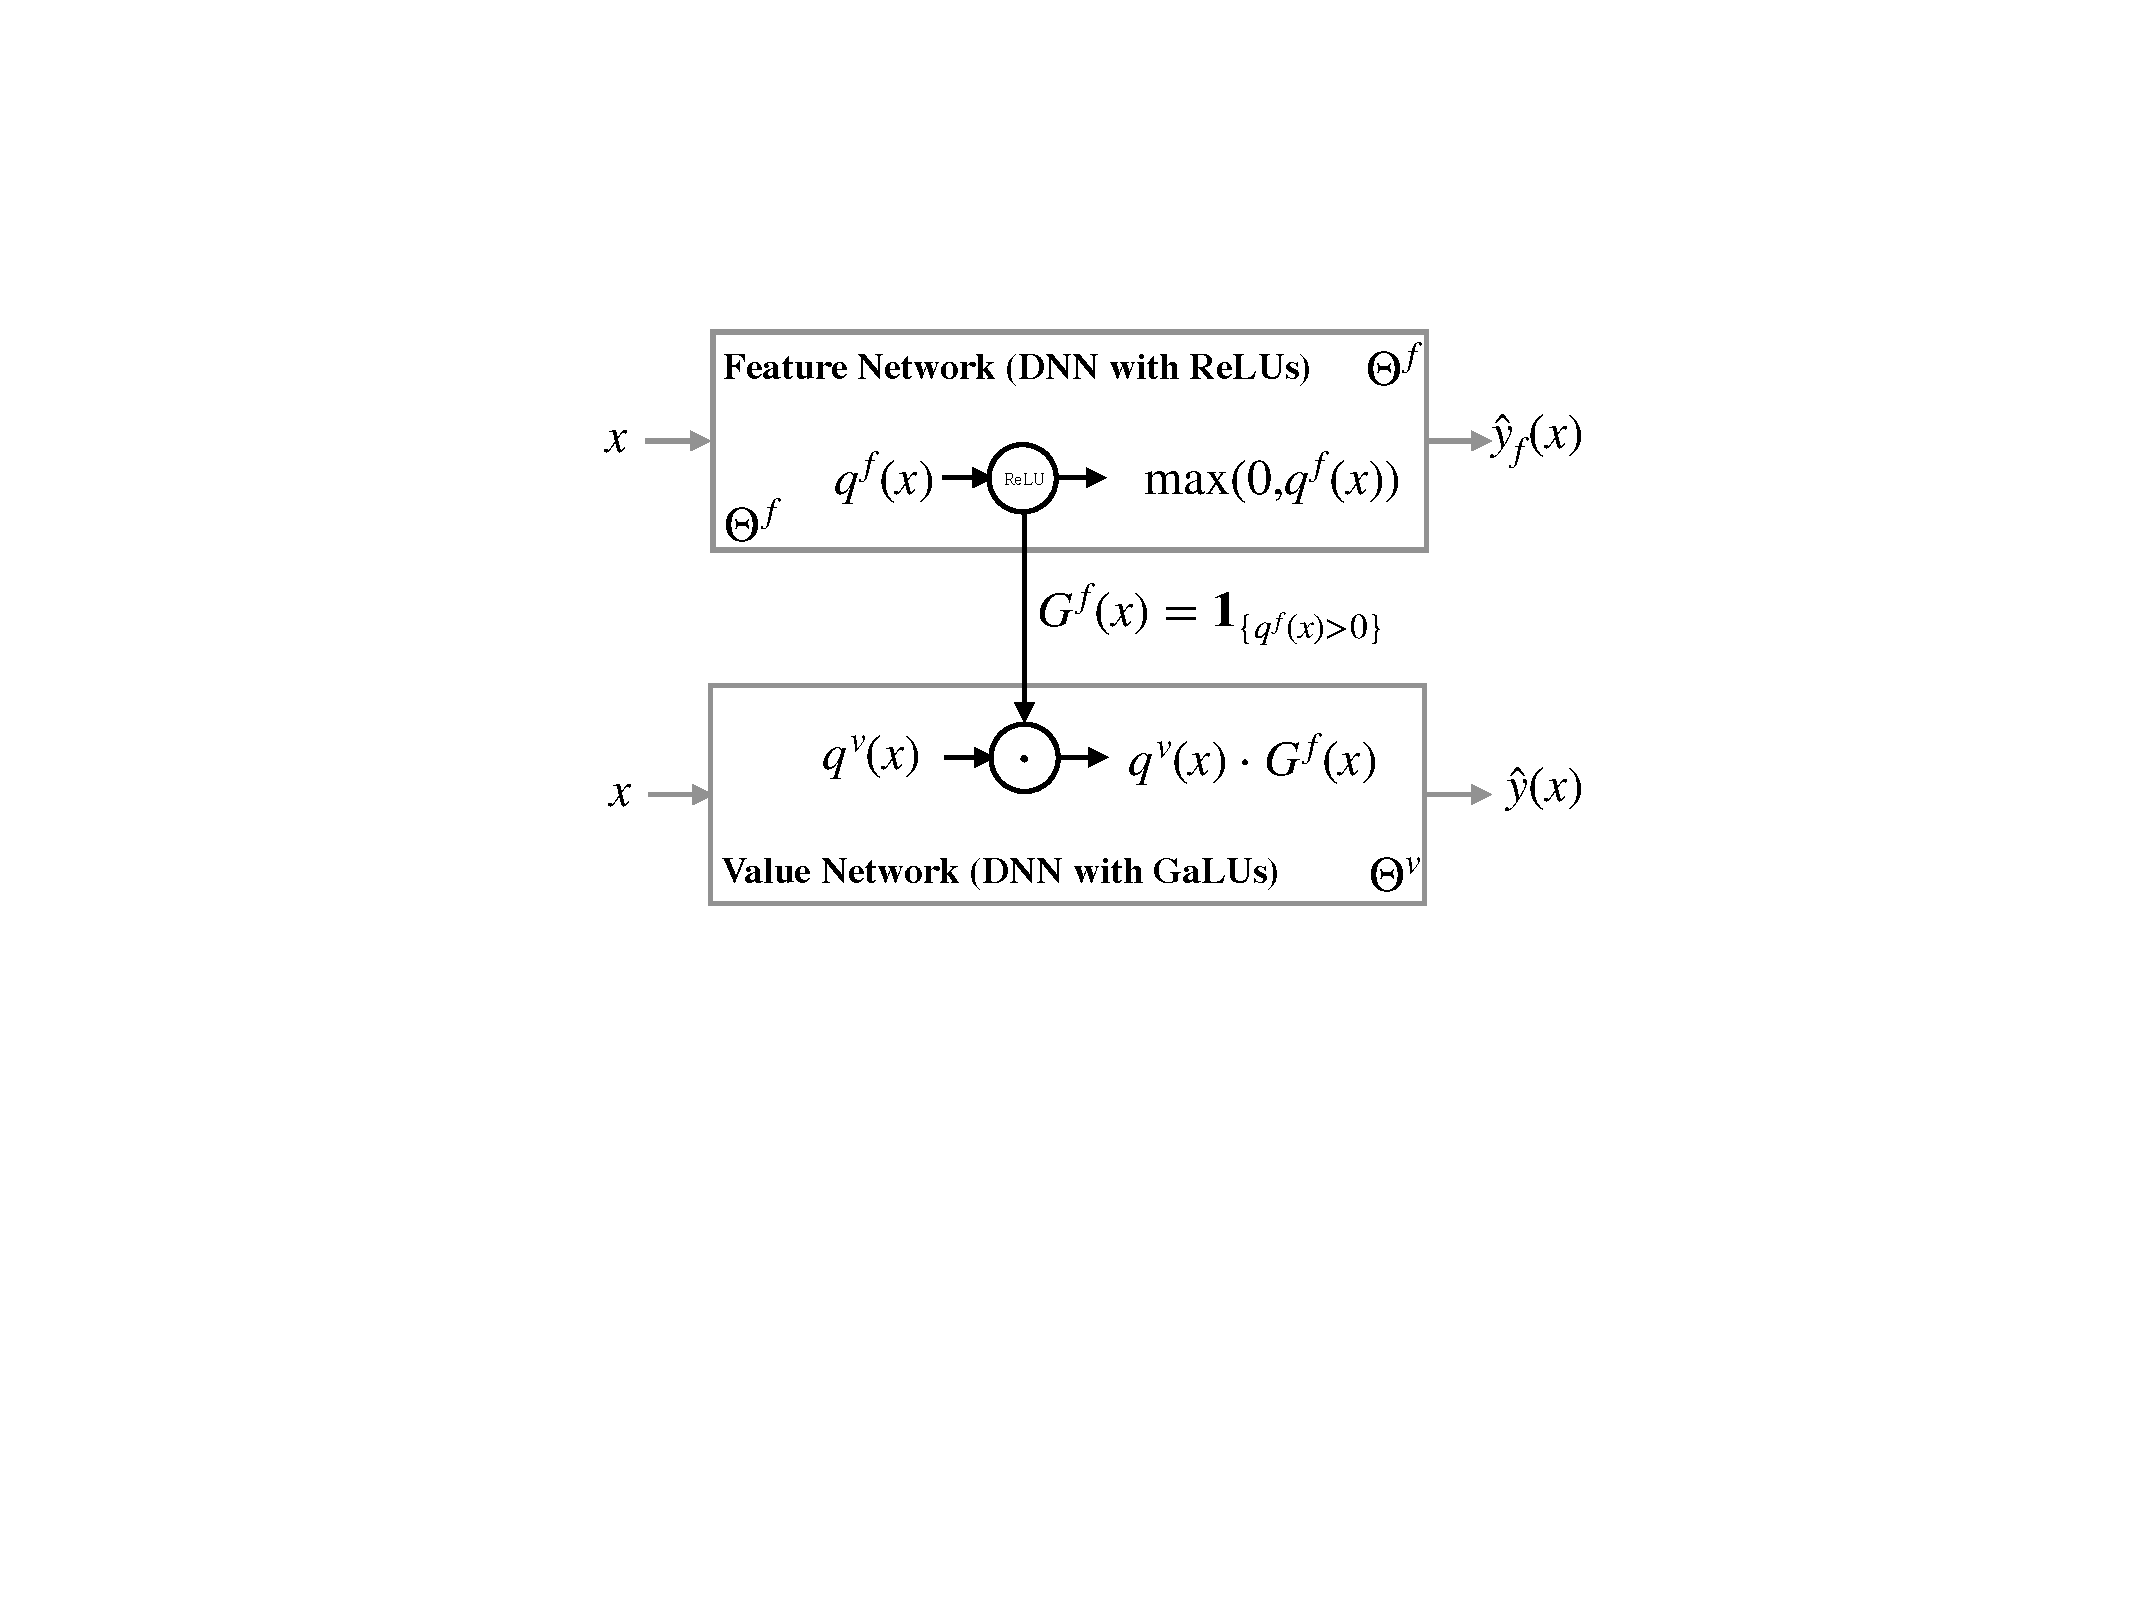
\includegraphics[scale=0.25]{figs/dgn-nips.pdf}
\caption{DGN}
\label{fig:dgn}
\end{wrapfigure}
\end{comment}

\begin{figure}[h]

\begin{minipage}{0.25\columnwidth}
\resizebox{\columnwidth}{!}{
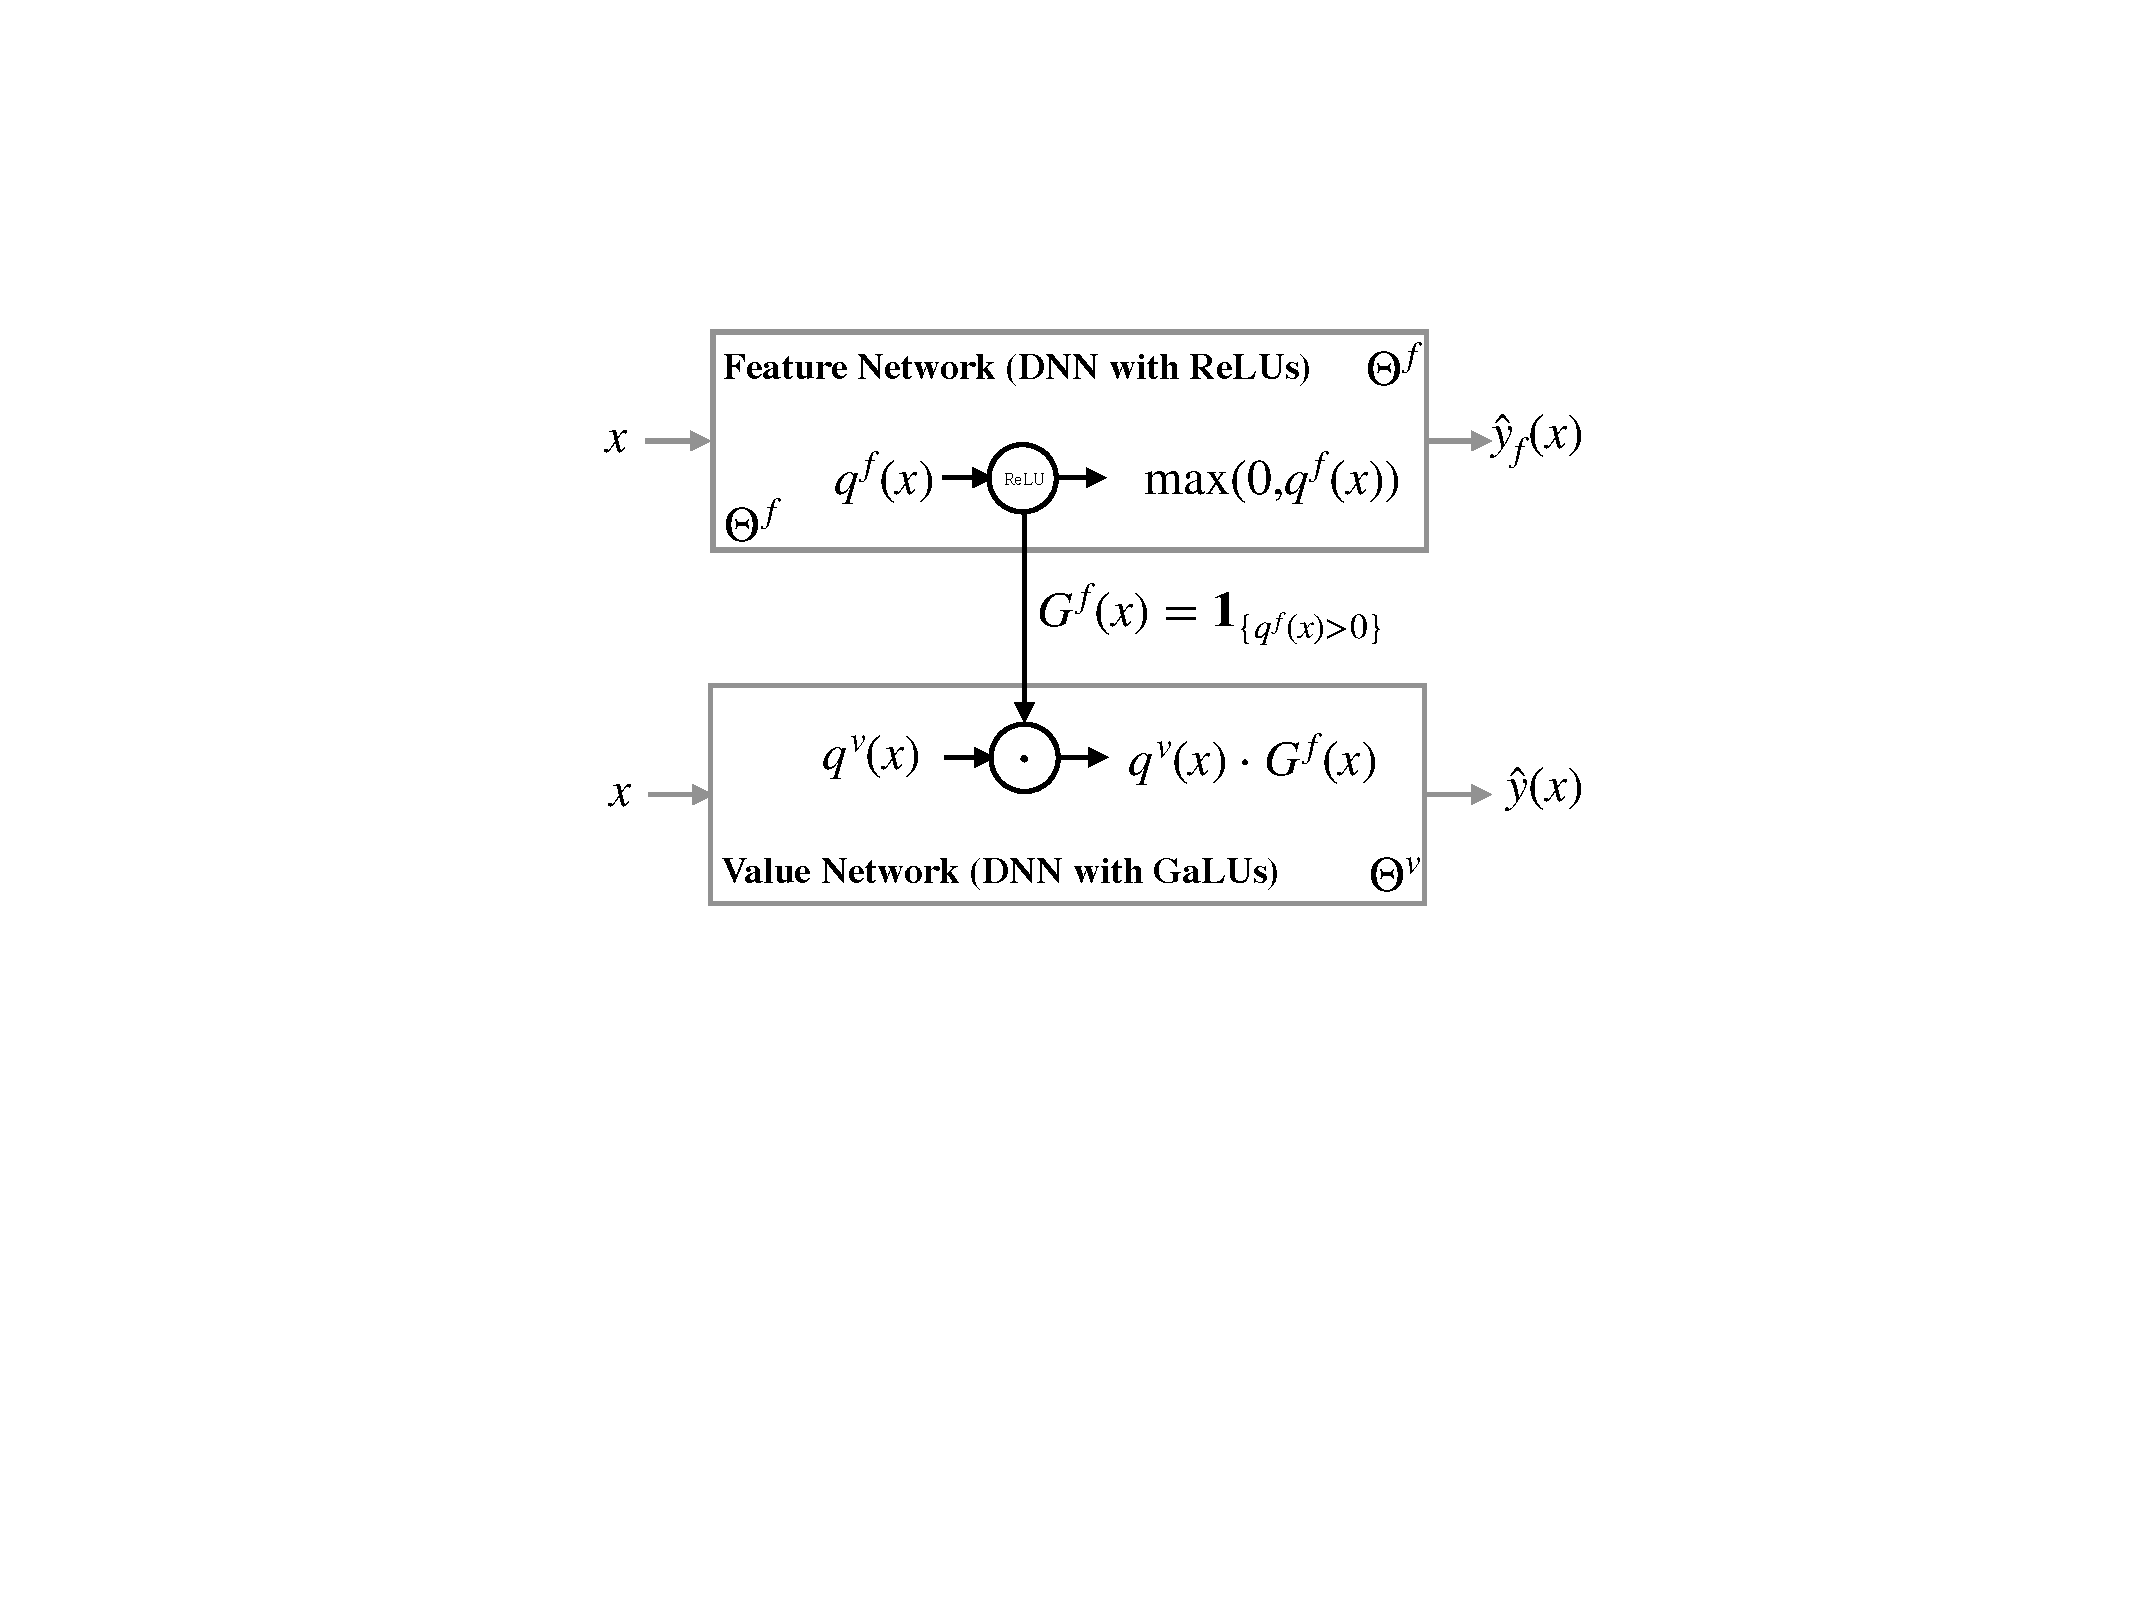
\includegraphics[scale=0.25]{figs/dgn-nips.pdf}
}
\end{minipage}
\begin{minipage}{0.73\columnwidth}
\resizebox{\columnwidth}{!}{
\begin{tabular}{|ll|}\hline
Feature Network & Value Network\\
$z_{x,\Theta}(0)=x$& $z_{x,\Theta}(0)=x$ \\
$q_{x,\Theta}(i,l)=\sum_{j} \Theta(i,j,l)\cdot z_{x,\Theta}(j,l-1)$& $q_{x,\Theta}(i,l)=\sum_{j} \Theta(i,j,l)\cdot z_{x,\Theta}(j,l-1)$\\
$G_{x,\Theta}(i,l)=\mathbbm{1}_{\{q_{x,\Theta}(i,l)>0\}}$& $G_{x,\Theta}(i,l)=\mathbbm{1}_{\{q_{x,\Theta}(i,l)>0\}}$\\
$z_{x,\Theta}(i,l)=q_{x,\Theta}(i,l)\cdot G_{x,\Theta}(i,l)$ & $z_{x,\Theta}(i,l)=q_{x,\Theta}(i,l)\cdot G_{x,\Theta}(i,l)$ \\
 $\hat{y}_{\Theta}(x)=\sum_{j\in[w]} \Theta(1,j,d-1)\cdot z_{x,\Theta}(j,d-1)$ & $\hat{y}_{\Theta}(x)=\sum_{j\in[w]} \Theta(1,j,d-1)\cdot z_{x,\Theta}(j,d-1)$\\\hline
\end{tabular}
}
\end{minipage}
\caption{DGN}
\label{fig:dgn}
\end{figure}

Note that since $\hat{y}_{\Theta}(x)=\ip{\phi_{x,\Theta},v_{\Theta}}$, during training, as $\Theta$ is learnt, both the NPFs and NPV are also learnt. Hence, in order to understand the roles of $\phi_{x,\Theta}$ and $v_{\Theta}$ it is a good idea to separate them. This is achieved by the deep gated network (DGN) setup (see \Cref{fig:dgn}), which has two networks namely the \emph{feature network} parameterised by $\Tf\in\R^{d^{\text{f}}_{\text{net}}}$ which holds the NPFs (i.e., the gating information) and a \emph{value network} parameterised by $\Tv\in\R^{d^{\text{v}}_{\text{net}}}$ which holds the NPV.  The combined parameterisation is denoted by $\Theta^{\text{DGN}}=(\Tf,\Tv)\in \R^{d^{\text{f}}_{\text{net}}+d^{\text{v}}_{\text{net}}}$.  


\begin{comment}
\FloatBarrier
\begin{figure}[h]
\begin{minipage}{0.35\columnwidth}
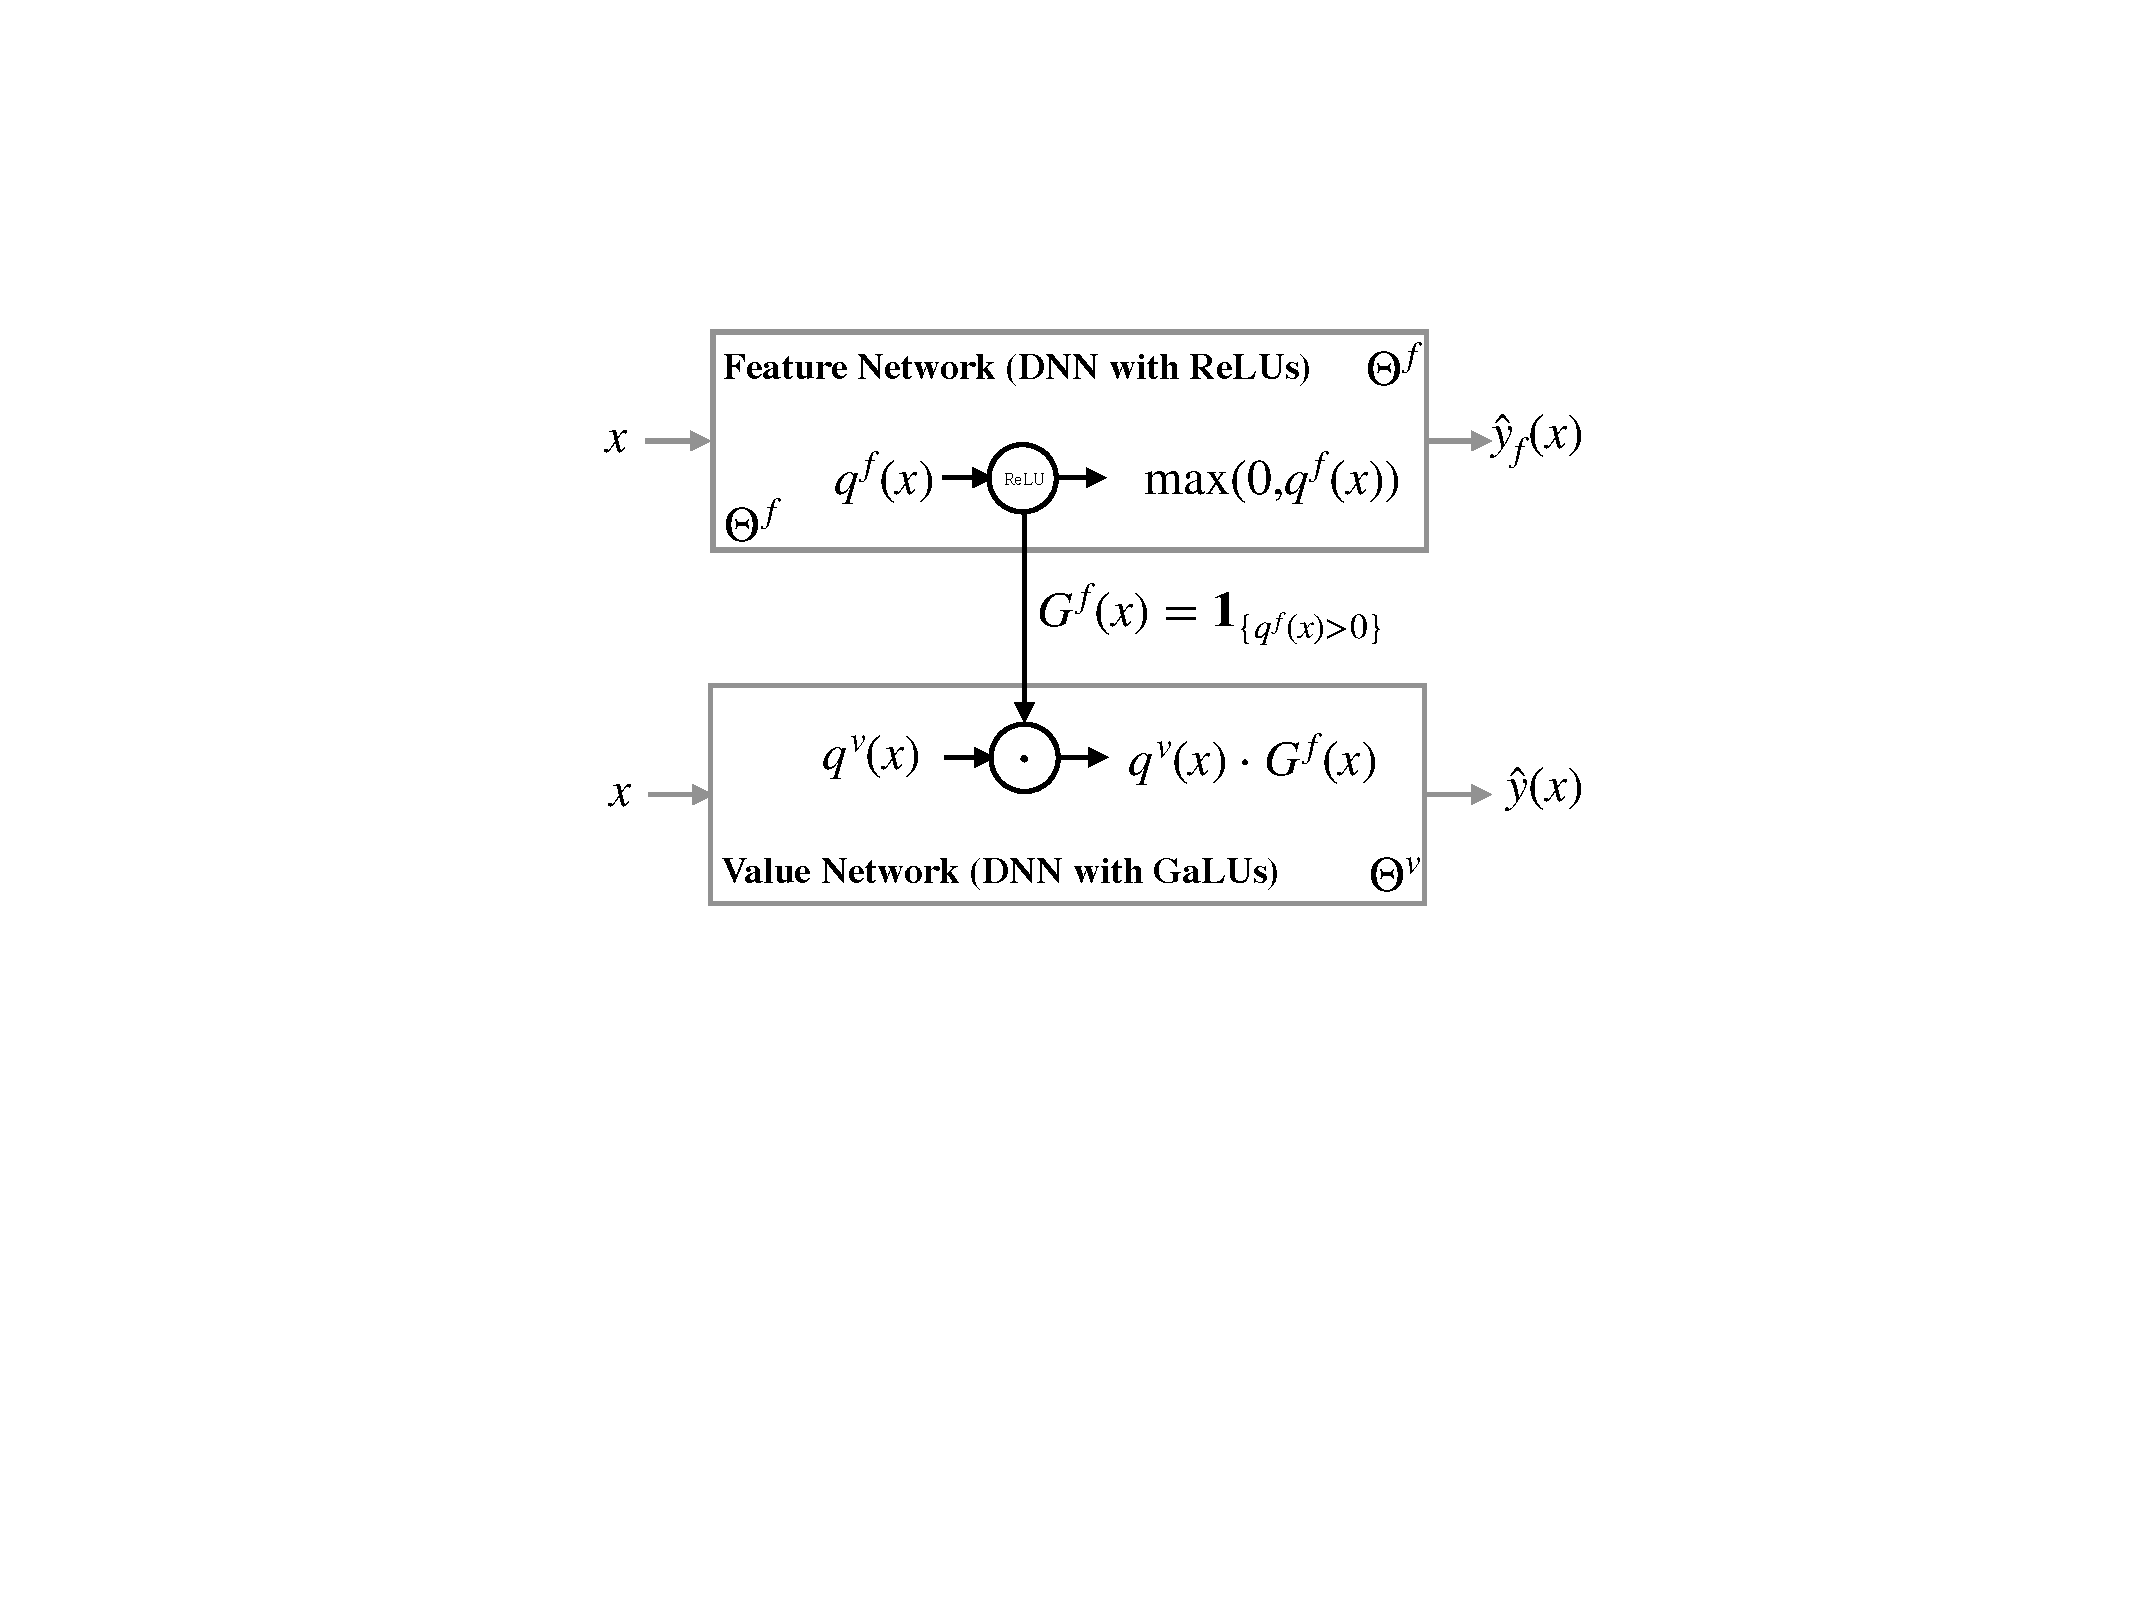
\includegraphics[scale=0.25]{figs/dgn-nips.pdf}
\end{minipage}
\begin{minipage}{0.6\columnwidth}
%\resizebox{\columnwidth}{!}{
\begin{tabular}{|c|c|}\hline
Regime & Feature Network \\\hline
Fixed Learnt & pre-trained; non-trainable \\\hline
Fixed Random & random; non-trainable\\\hline
Decoupled Learning & trainable \\\hline
\end{tabular}
%}
%\begin{tabular}{|c|c|}\hline
%Gating & Expression \\\hline
%Hard & $G^\text{f}(x) = \mathbf{1}_{\{q^{\text{f}}(x)>0\}}$ \\\hline
%Soft &  $G^\text{f}(x) = 1/(1+\exp{-\beta q^{\text{f}}(x)})$\\\hline
%\end{tabular}
%\resizebox{\columnwidth}{!}{
%\begin{tabular}{|c|c|}\hline
%NTK & $K_{\Tdgn}(x,x')=\ip{\nabla_{\Tdgn}\hat{y}(x),\nabla_{\Tdgn}\hat{y}(x')}$\\\hline
%Kernel & Expression\\\hline
%$\text{NTK}^{\text{gate-learn}}:$ & $\kf_{\Tdgn}(x,x')=\ip{ \nabla_{\Tf}\hat{y}(x), \nabla_{\Tf}\hat{y}(x') }$\\\hline
%$\text{NTK}^{\text{fixed-gate}}:$ & $\kv_{\Tdgn}(x,x')=\ip{ \nabla_{\Tv}\hat{y}(x), \nabla_{\Tv}\hat{y}(x') }$,\\\hline
%\end{tabular}
%}
\end{minipage}
\caption{Deep Gated Network }
\label{fig:dgn}
\end{figure}
\end{comment}
\begin{proposition}\label{prop:ntks} Let $\kv_{\Tdgn}(x,x')=\ip{ \nabla_{\Tv}\hat{y}(x), \nabla_{\Tv}\hat{y}(x')}$, and  $\kf_{\Tdgn}(x,x')=\ip{ \nabla_{\Tf}\hat{y}(x), \nabla_{\Tf}\hat{y}(x') }$ and $K_{\Tdgn}$ be the NTK matrix of the DGN. Then 
\begin{align*}
K_{\Tdgn}=\kv_{\Tdgn}+\kf_{\Tdgn}
\end{align*}

\end{proposition}
\textbf{Remark:} In the case of fixed regimes, $\kf_{\Tdgn}=0$. 

\subsection{Overlap of Sub-Networks and Neural Path Kernel}

\begin{definition}\label{def:cnnlambda}
The total number of `active' paths for both $x$ and $x'$ that pass through input node $i$ is defined to be:\\
{\centering{$\textbf{overlap}_{\Theta}(i,x,x') = \Lambda_{\Theta}(i,x,x') \eqdef \left|\{p\in[P]\colon  \Ifeat_0(p)=i, A_{\Theta}(x,p)= A_{\Theta}(x',p)=1\}\right|$}}
\end{definition}
%\subsection{NPK of FC-DNN: Product Kernel }
%\input{cnpkexample}
%\subsection{Neural Path Kernel : Similarity based on active sub-networks}
\begin{definition}
Let $D\in\R^{\din}$ be a vector of non-negative entries  and for $u,u'\in\R^{\din}$ , let $\ip{u,u'}_{D}=\sum_{i=1}^{\din}D(i)u(i)u'(i)$. 
\end{definition}

\begin{lemma}
Let $H_{\Theta}(x,x')\eqdef\langle\phi_{x,\Theta},\phi_{x',\Theta} \rangle$ be the NPK. Then  
\begin{align*} 
H_{\Theta}(x,x')=\ip{x,x'}_{\Lambda_{\Theta}(\cdot,x,x')} 
\end{align*}
\end{lemma}

\subsection{NTK $\propto$ NPK}
\begin{assumption}\label{assmp:main}
(i) $\Tv_0$ is statistically independent of $\Tf_0$ (ii) $\Tv_0$ are i.i.d symmetric Bernoulli over $\{-{\sigma},+{\sigma}\}$. 
\end{assumption}

\begin{theorem}\label{th:main} Let $\sigma=\frac{\cscale}{\sqrt{w}}$. Under \Cref{assmp:main}, a $w\ra\infty$, for FC-DGN we have: 
\begin{align*}
\kv_{\Tdgn_0}(x,x') &\ra d\cdot \sigma^{d-1}\cdot H_{\Tf_0}(x,x')= d\cdot \sigma^{d-1}\cdot \ip{x,x'}_{\Lambda_{\Tf_0}(\cdot,x,x')}  \\
\end{align*}
\end{theorem}
\begin{figure}[h]
\begin{minipage}{0.49\columnwidth}
\resizebox{\columnwidth}{!}{
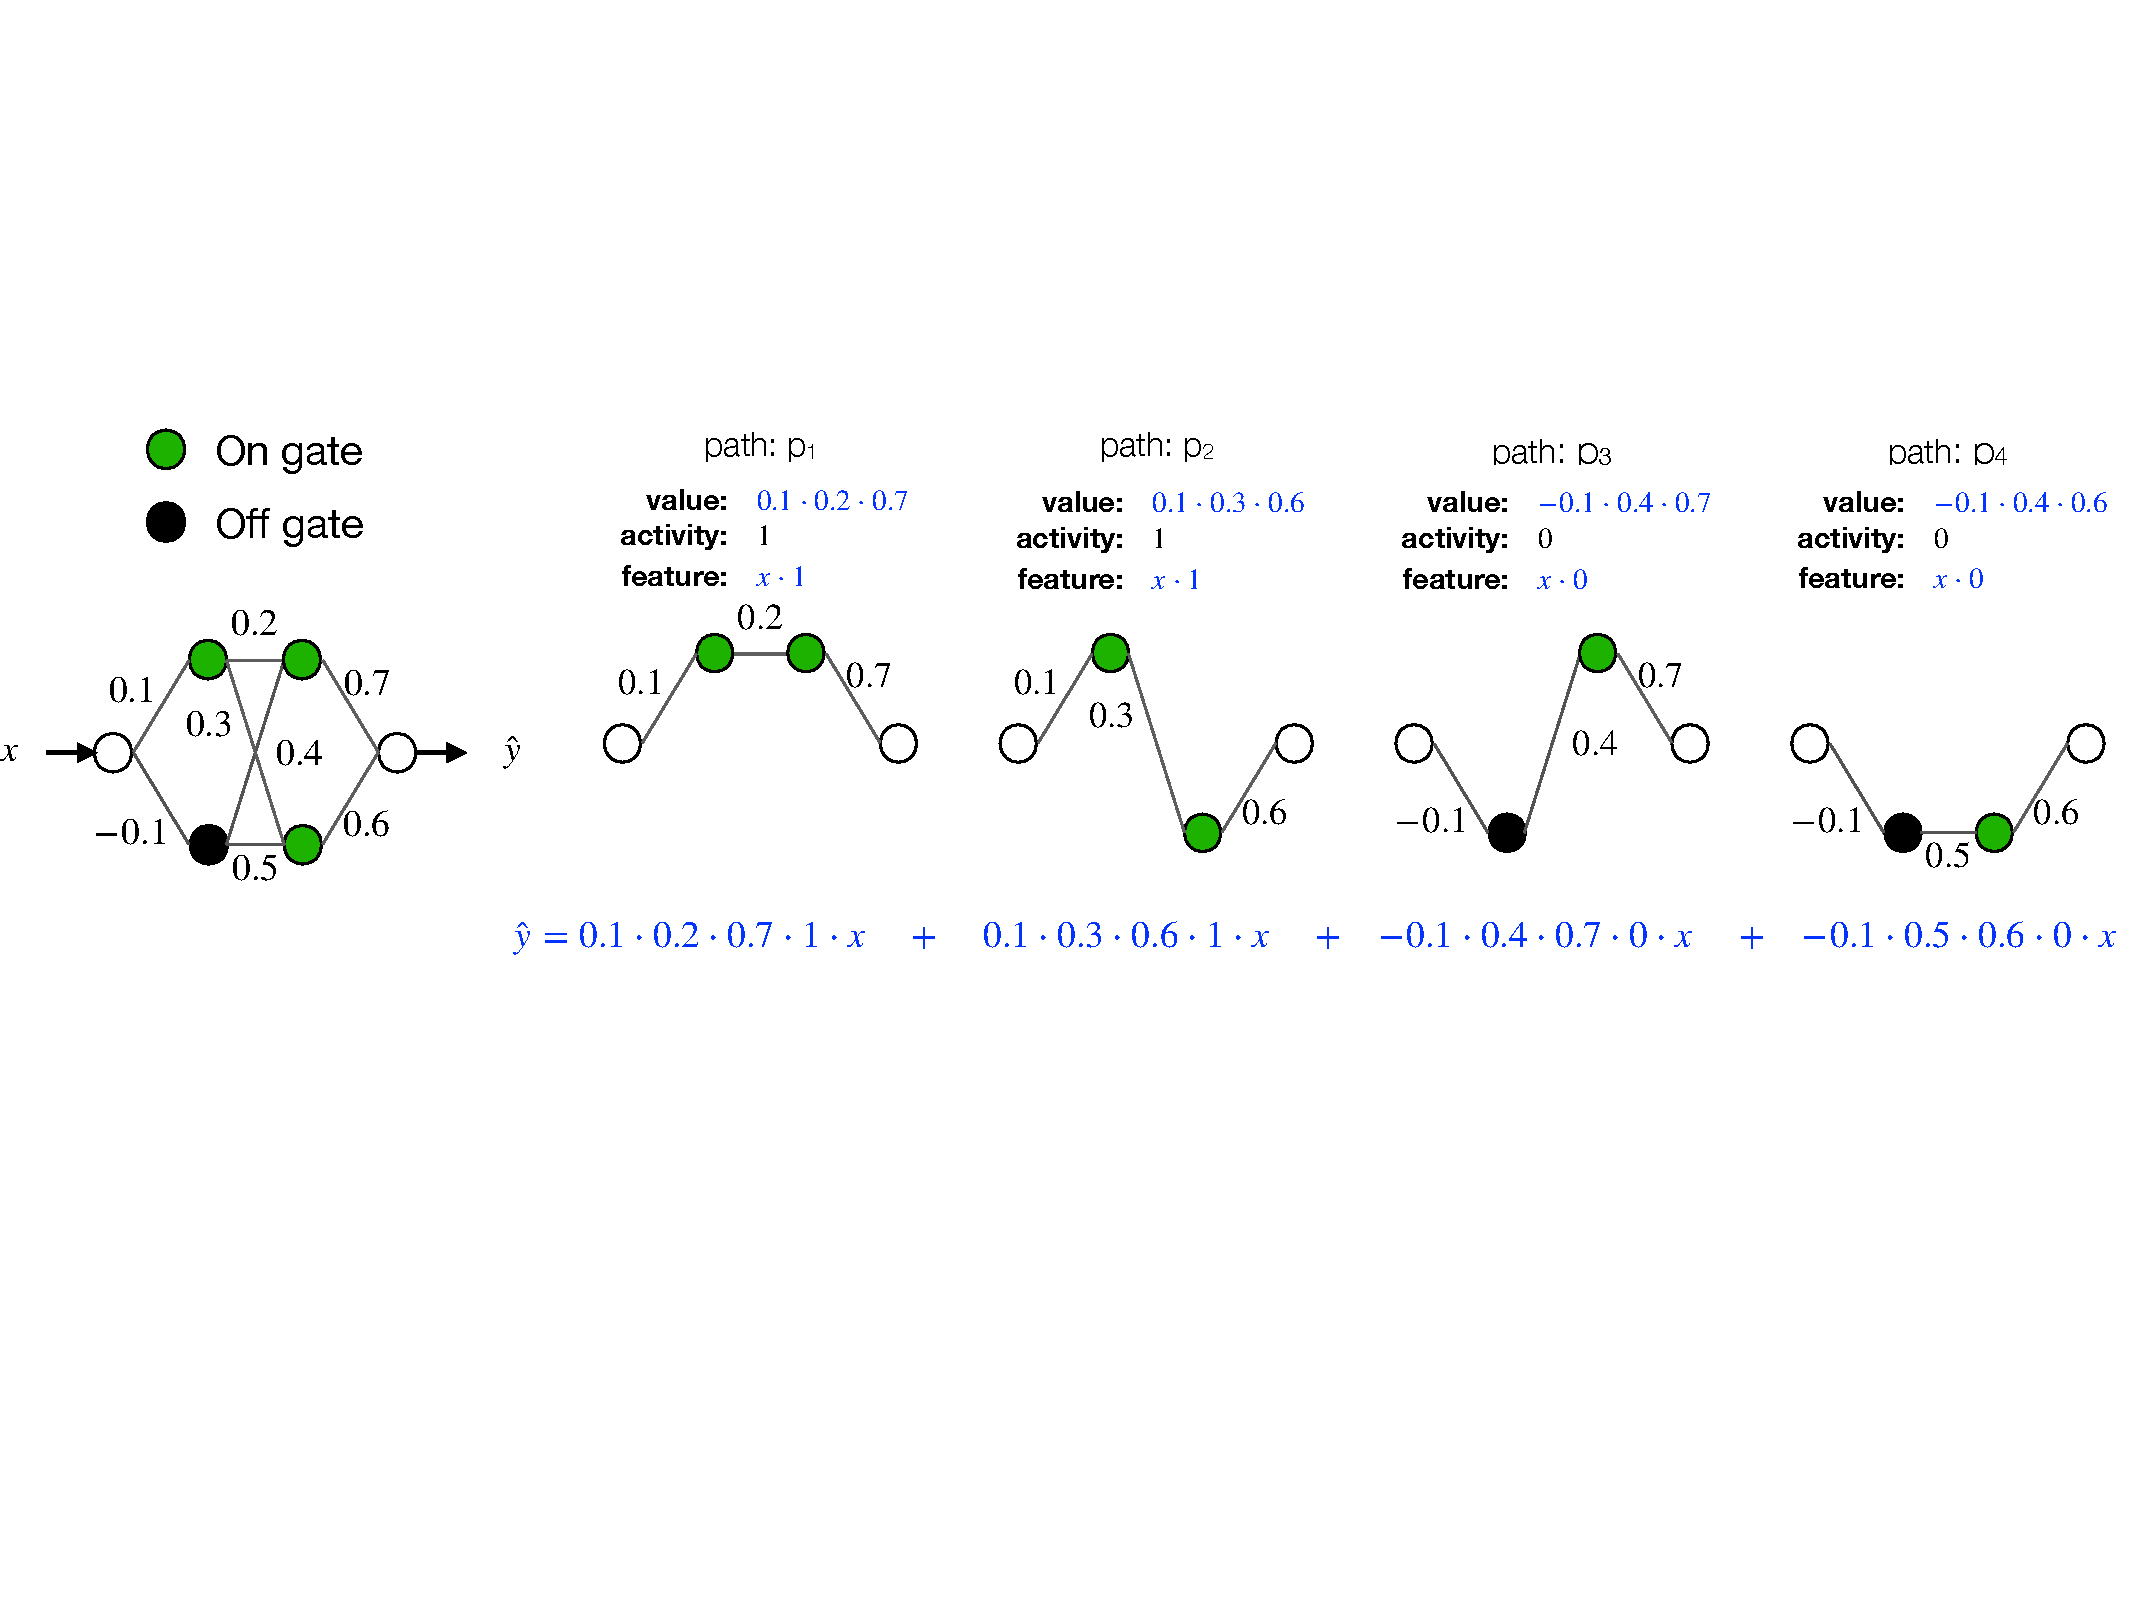
\includegraphics[scale=0.5]{figs/overlap.pdf}
}
\end{minipage}
\begin{minipage}{0.49\columnwidth}
\resizebox{\columnwidth}{!}{
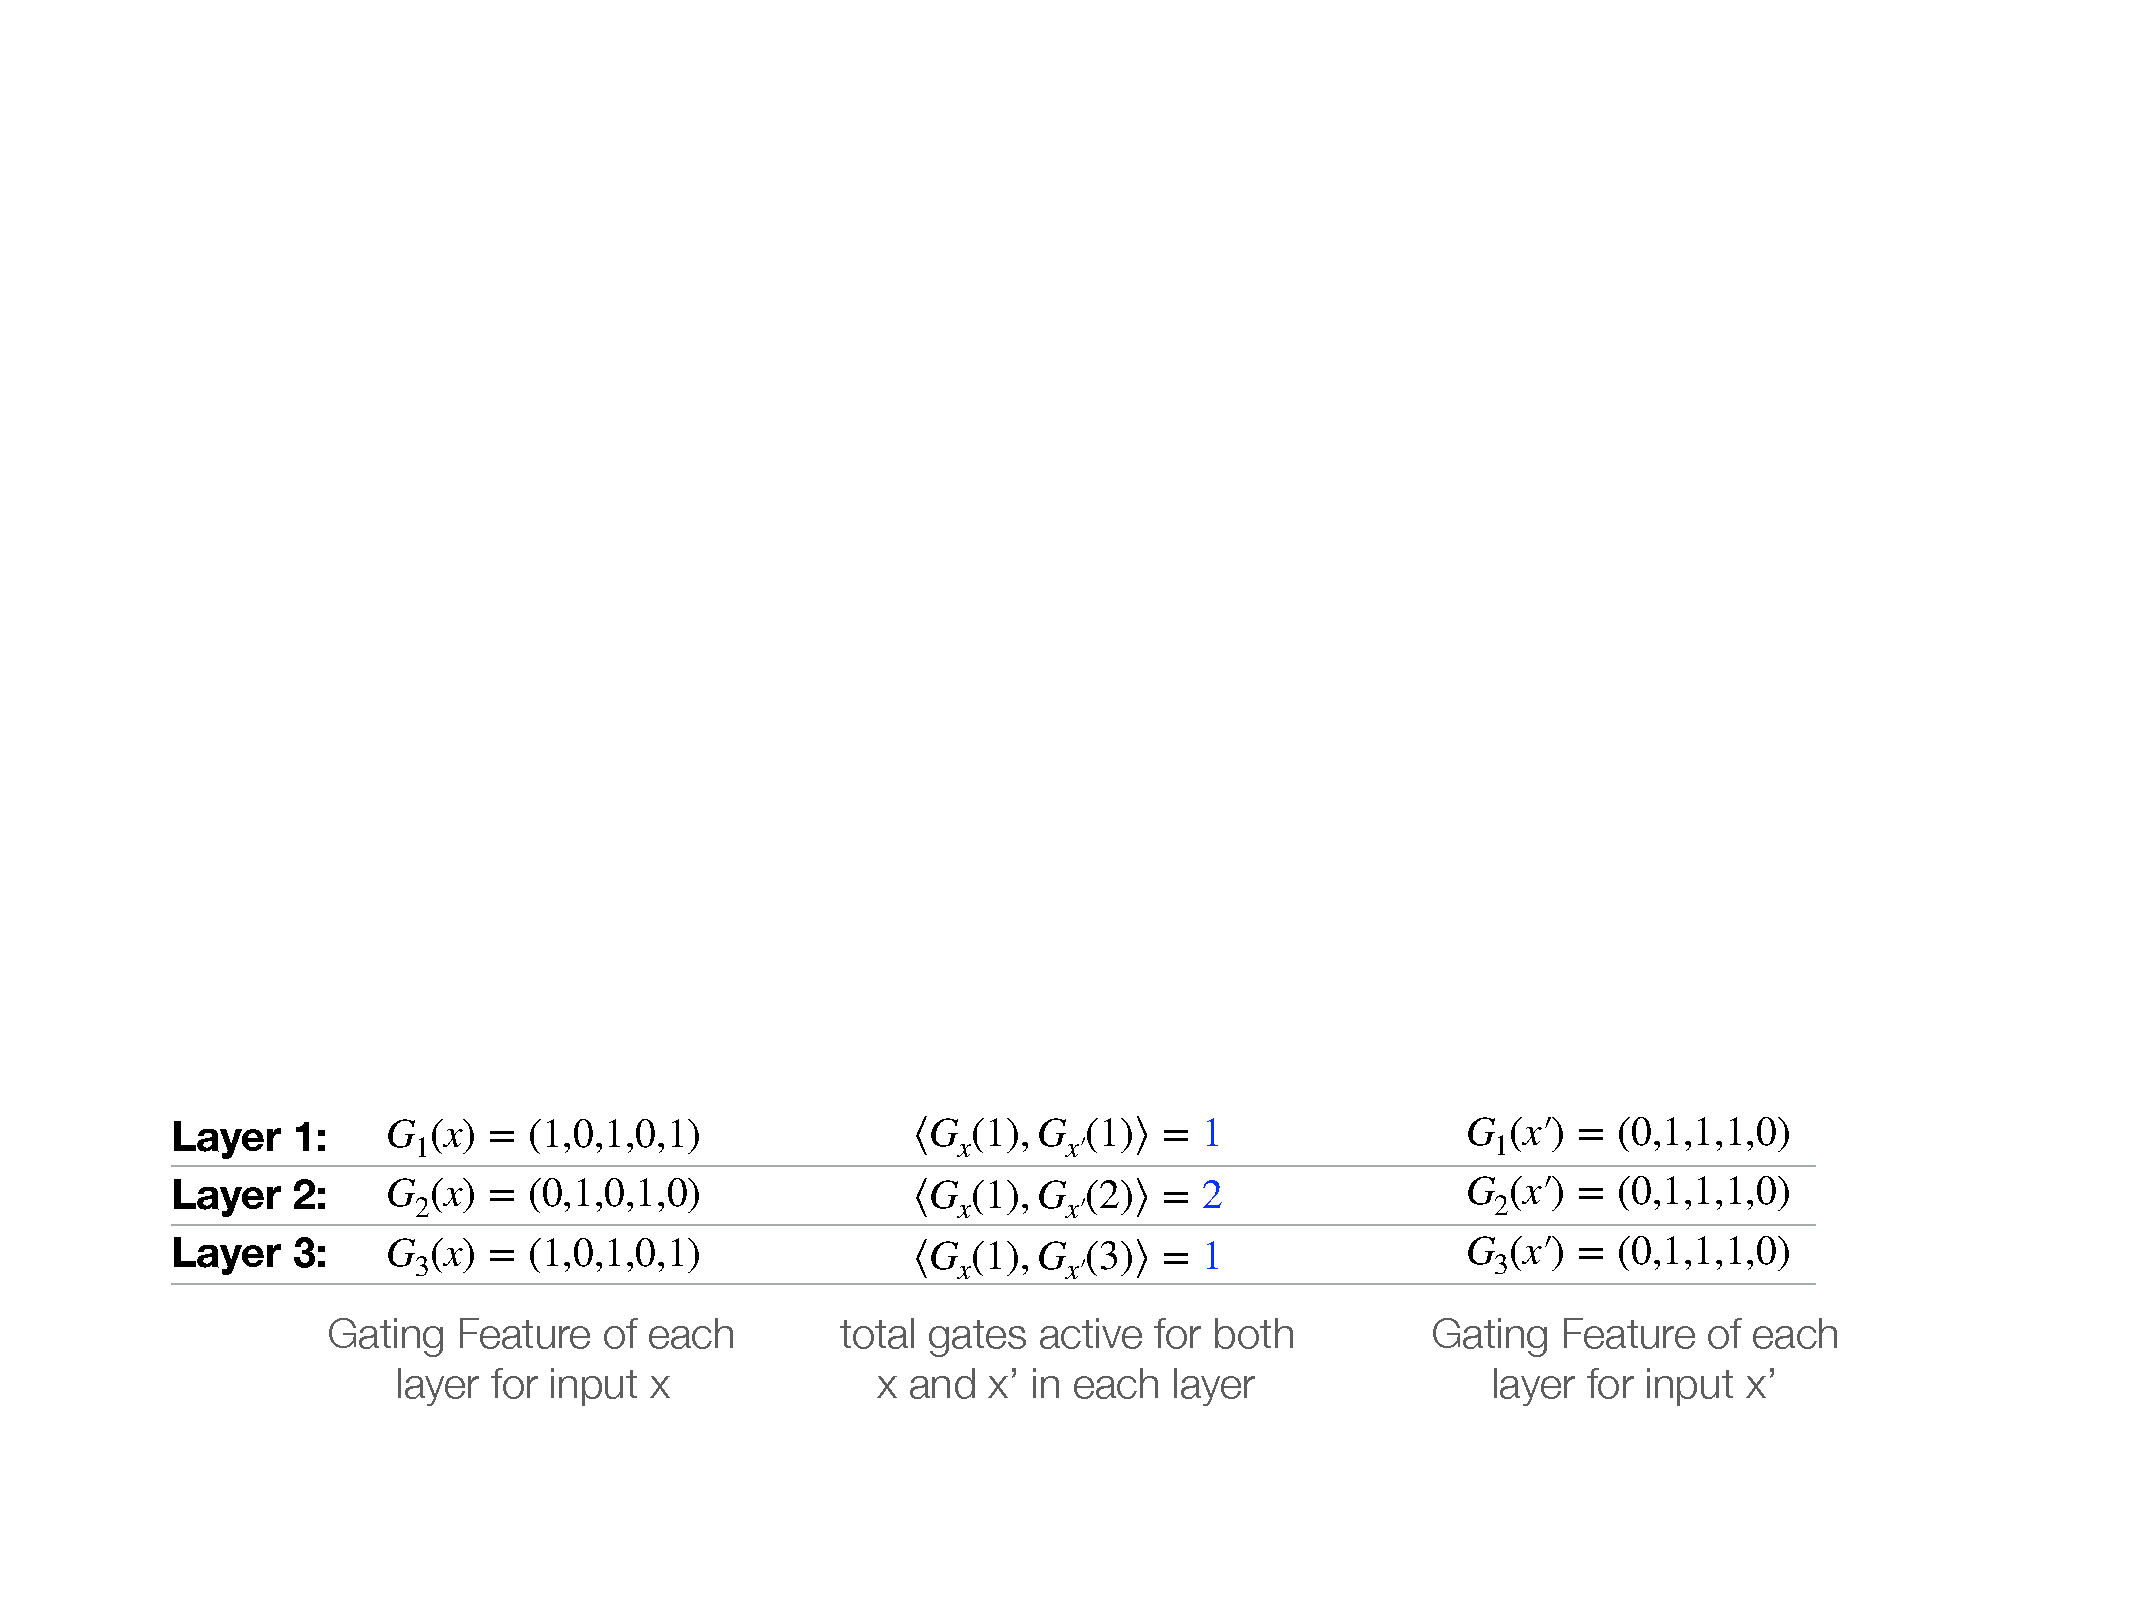
\includegraphics[scale=0.5]{figs/gating-features.pdf}
}
\end{minipage}
\caption{Shows a toy illustration of active sub-networks for two inputs $x$ and $x'$ and the common overlapping sub-network. The total number of active paths from any input node $i$, $\Lambda(i,x,')=\Pi_{i=1}^{3} \ip{G_l(x),G_l(x'}=1\cdot 2\cdot 1 =2$.}
\label{fig:overlap}
\end{figure}
